
% Default to the notebook output style

    


% Inherit from the specified cell style.




    
\documentclass{article}

    
    
    \usepackage{graphicx} % Used to insert images
    \usepackage{adjustbox} % Used to constrain images to a maximum size 
    \usepackage{color} % Allow colors to be defined
    \usepackage{enumerate} % Needed for markdown enumerations to work
    \usepackage{geometry} % Used to adjust the document margins
    \usepackage{amsmath} % Equations
    \usepackage{amssymb} % Equations
    \usepackage[mathletters]{ucs} % Extended unicode (utf-8) support
    \usepackage[utf8x]{inputenc} % Allow utf-8 characters in the tex document
    \usepackage{fancyvrb} % verbatim replacement that allows latex
    \usepackage{grffile} % extends the file name processing of package graphics 
                         % to support a larger range 
    % The hyperref package gives us a pdf with properly built
    % internal navigation ('pdf bookmarks' for the table of contents,
    % internal cross-reference links, web links for URLs, etc.)
    \usepackage{hyperref}
    \usepackage{longtable} % longtable support required by pandoc >1.10
    

    
    
    \definecolor{orange}{cmyk}{0,0.4,0.8,0.2}
    \definecolor{darkorange}{rgb}{.71,0.21,0.01}
    \definecolor{darkgreen}{rgb}{.12,.54,.11}
    \definecolor{myteal}{rgb}{.26, .44, .56}
    \definecolor{gray}{gray}{0.45}
    \definecolor{lightgray}{gray}{.95}
    \definecolor{mediumgray}{gray}{.8}
    \definecolor{inputbackground}{rgb}{.95, .95, .85}
    \definecolor{outputbackground}{rgb}{.95, .95, .95}
    \definecolor{traceback}{rgb}{1, .95, .95}
    % ansi colors
    \definecolor{red}{rgb}{.6,0,0}
    \definecolor{green}{rgb}{0,.65,0}
    \definecolor{brown}{rgb}{0.6,0.6,0}
    \definecolor{blue}{rgb}{0,.145,.698}
    \definecolor{purple}{rgb}{.698,.145,.698}
    \definecolor{cyan}{rgb}{0,.698,.698}
    \definecolor{lightgray}{gray}{0.5}
    
    % bright ansi colors
    \definecolor{darkgray}{gray}{0.25}
    \definecolor{lightred}{rgb}{1.0,0.39,0.28}
    \definecolor{lightgreen}{rgb}{0.48,0.99,0.0}
    \definecolor{lightblue}{rgb}{0.53,0.81,0.92}
    \definecolor{lightpurple}{rgb}{0.87,0.63,0.87}
    \definecolor{lightcyan}{rgb}{0.5,1.0,0.83}
    
    % commands and environments needed by pandoc snippets
    % extracted from the output of `pandoc -s`
    
    \DefineShortVerb[commandchars=\\\{\}]{\|}
    \DefineVerbatimEnvironment{Highlighting}{Verbatim}{commandchars=\\\{\}}
    % Add ',fontsize=\small' for more characters per line
    \newenvironment{Shaded}{}{}
    \newcommand{\KeywordTok}[1]{\textcolor[rgb]{0.00,0.44,0.13}{\textbf{{#1}}}}
    \newcommand{\DataTypeTok}[1]{\textcolor[rgb]{0.56,0.13,0.00}{{#1}}}
    \newcommand{\DecValTok}[1]{\textcolor[rgb]{0.25,0.63,0.44}{{#1}}}
    \newcommand{\BaseNTok}[1]{\textcolor[rgb]{0.25,0.63,0.44}{{#1}}}
    \newcommand{\FloatTok}[1]{\textcolor[rgb]{0.25,0.63,0.44}{{#1}}}
    \newcommand{\CharTok}[1]{\textcolor[rgb]{0.25,0.44,0.63}{{#1}}}
    \newcommand{\StringTok}[1]{\textcolor[rgb]{0.25,0.44,0.63}{{#1}}}
    \newcommand{\CommentTok}[1]{\textcolor[rgb]{0.38,0.63,0.69}{\textit{{#1}}}}
    \newcommand{\OtherTok}[1]{\textcolor[rgb]{0.00,0.44,0.13}{{#1}}}
    \newcommand{\AlertTok}[1]{\textcolor[rgb]{1.00,0.00,0.00}{\textbf{{#1}}}}
    \newcommand{\FunctionTok}[1]{\textcolor[rgb]{0.02,0.16,0.49}{{#1}}}
    \newcommand{\RegionMarkerTok}[1]{{#1}}
    \newcommand{\ErrorTok}[1]{\textcolor[rgb]{1.00,0.00,0.00}{\textbf{{#1}}}}
    \newcommand{\NormalTok}[1]{{#1}}
    
    % Define a nice break command that doesn't care if a line doesn't already
    % exist.
    \def\br{\hspace*{\fill} \\* }
    % Math Jax compatability definitions
    \def\gt{>}
    \def\lt{<}
    % Document parameters
    \title{Transitor de Unio?n Bipolar (BJT)}
    
    
    

    % Pygments definitions
    
\makeatletter
\def\PY@reset{\let\PY@it=\relax \let\PY@bf=\relax%
    \let\PY@ul=\relax \let\PY@tc=\relax%
    \let\PY@bc=\relax \let\PY@ff=\relax}
\def\PY@tok#1{\csname PY@tok@#1\endcsname}
\def\PY@toks#1+{\ifx\relax#1\empty\else%
    \PY@tok{#1}\expandafter\PY@toks\fi}
\def\PY@do#1{\PY@bc{\PY@tc{\PY@ul{%
    \PY@it{\PY@bf{\PY@ff{#1}}}}}}}
\def\PY#1#2{\PY@reset\PY@toks#1+\relax+\PY@do{#2}}

\expandafter\def\csname PY@tok@si\endcsname{\let\PY@bf=\textbf\def\PY@tc##1{\textcolor[rgb]{0.73,0.40,0.53}{##1}}}
\expandafter\def\csname PY@tok@sh\endcsname{\def\PY@tc##1{\textcolor[rgb]{0.73,0.13,0.13}{##1}}}
\expandafter\def\csname PY@tok@ni\endcsname{\let\PY@bf=\textbf\def\PY@tc##1{\textcolor[rgb]{0.60,0.60,0.60}{##1}}}
\expandafter\def\csname PY@tok@nn\endcsname{\let\PY@bf=\textbf\def\PY@tc##1{\textcolor[rgb]{0.00,0.00,1.00}{##1}}}
\expandafter\def\csname PY@tok@no\endcsname{\def\PY@tc##1{\textcolor[rgb]{0.53,0.00,0.00}{##1}}}
\expandafter\def\csname PY@tok@nl\endcsname{\def\PY@tc##1{\textcolor[rgb]{0.63,0.63,0.00}{##1}}}
\expandafter\def\csname PY@tok@c1\endcsname{\let\PY@it=\textit\def\PY@tc##1{\textcolor[rgb]{0.25,0.50,0.50}{##1}}}
\expandafter\def\csname PY@tok@nc\endcsname{\let\PY@bf=\textbf\def\PY@tc##1{\textcolor[rgb]{0.00,0.00,1.00}{##1}}}
\expandafter\def\csname PY@tok@sc\endcsname{\def\PY@tc##1{\textcolor[rgb]{0.73,0.13,0.13}{##1}}}
\expandafter\def\csname PY@tok@na\endcsname{\def\PY@tc##1{\textcolor[rgb]{0.49,0.56,0.16}{##1}}}
\expandafter\def\csname PY@tok@nf\endcsname{\def\PY@tc##1{\textcolor[rgb]{0.00,0.00,1.00}{##1}}}
\expandafter\def\csname PY@tok@sd\endcsname{\let\PY@it=\textit\def\PY@tc##1{\textcolor[rgb]{0.73,0.13,0.13}{##1}}}
\expandafter\def\csname PY@tok@nd\endcsname{\def\PY@tc##1{\textcolor[rgb]{0.67,0.13,1.00}{##1}}}
\expandafter\def\csname PY@tok@ne\endcsname{\let\PY@bf=\textbf\def\PY@tc##1{\textcolor[rgb]{0.82,0.25,0.23}{##1}}}
\expandafter\def\csname PY@tok@sx\endcsname{\def\PY@tc##1{\textcolor[rgb]{0.00,0.50,0.00}{##1}}}
\expandafter\def\csname PY@tok@sb\endcsname{\def\PY@tc##1{\textcolor[rgb]{0.73,0.13,0.13}{##1}}}
\expandafter\def\csname PY@tok@ss\endcsname{\def\PY@tc##1{\textcolor[rgb]{0.10,0.09,0.49}{##1}}}
\expandafter\def\csname PY@tok@sr\endcsname{\def\PY@tc##1{\textcolor[rgb]{0.73,0.40,0.53}{##1}}}
\expandafter\def\csname PY@tok@nv\endcsname{\def\PY@tc##1{\textcolor[rgb]{0.10,0.09,0.49}{##1}}}
\expandafter\def\csname PY@tok@nt\endcsname{\let\PY@bf=\textbf\def\PY@tc##1{\textcolor[rgb]{0.00,0.50,0.00}{##1}}}
\expandafter\def\csname PY@tok@m\endcsname{\def\PY@tc##1{\textcolor[rgb]{0.40,0.40,0.40}{##1}}}
\expandafter\def\csname PY@tok@o\endcsname{\def\PY@tc##1{\textcolor[rgb]{0.40,0.40,0.40}{##1}}}
\expandafter\def\csname PY@tok@vi\endcsname{\def\PY@tc##1{\textcolor[rgb]{0.10,0.09,0.49}{##1}}}
\expandafter\def\csname PY@tok@k\endcsname{\let\PY@bf=\textbf\def\PY@tc##1{\textcolor[rgb]{0.00,0.50,0.00}{##1}}}
\expandafter\def\csname PY@tok@gr\endcsname{\def\PY@tc##1{\textcolor[rgb]{1.00,0.00,0.00}{##1}}}
\expandafter\def\csname PY@tok@c\endcsname{\let\PY@it=\textit\def\PY@tc##1{\textcolor[rgb]{0.25,0.50,0.50}{##1}}}
\expandafter\def\csname PY@tok@nb\endcsname{\def\PY@tc##1{\textcolor[rgb]{0.00,0.50,0.00}{##1}}}
\expandafter\def\csname PY@tok@mf\endcsname{\def\PY@tc##1{\textcolor[rgb]{0.40,0.40,0.40}{##1}}}
\expandafter\def\csname PY@tok@se\endcsname{\let\PY@bf=\textbf\def\PY@tc##1{\textcolor[rgb]{0.73,0.40,0.13}{##1}}}
\expandafter\def\csname PY@tok@w\endcsname{\def\PY@tc##1{\textcolor[rgb]{0.73,0.73,0.73}{##1}}}
\expandafter\def\csname PY@tok@kc\endcsname{\let\PY@bf=\textbf\def\PY@tc##1{\textcolor[rgb]{0.00,0.50,0.00}{##1}}}
\expandafter\def\csname PY@tok@s\endcsname{\def\PY@tc##1{\textcolor[rgb]{0.73,0.13,0.13}{##1}}}
\expandafter\def\csname PY@tok@ow\endcsname{\let\PY@bf=\textbf\def\PY@tc##1{\textcolor[rgb]{0.67,0.13,1.00}{##1}}}
\expandafter\def\csname PY@tok@il\endcsname{\def\PY@tc##1{\textcolor[rgb]{0.40,0.40,0.40}{##1}}}
\expandafter\def\csname PY@tok@kd\endcsname{\let\PY@bf=\textbf\def\PY@tc##1{\textcolor[rgb]{0.00,0.50,0.00}{##1}}}
\expandafter\def\csname PY@tok@cp\endcsname{\def\PY@tc##1{\textcolor[rgb]{0.74,0.48,0.00}{##1}}}
\expandafter\def\csname PY@tok@cs\endcsname{\let\PY@it=\textit\def\PY@tc##1{\textcolor[rgb]{0.25,0.50,0.50}{##1}}}
\expandafter\def\csname PY@tok@err\endcsname{\def\PY@bc##1{\setlength{\fboxsep}{0pt}\fcolorbox[rgb]{1.00,0.00,0.00}{1,1,1}{\strut ##1}}}
\expandafter\def\csname PY@tok@kn\endcsname{\let\PY@bf=\textbf\def\PY@tc##1{\textcolor[rgb]{0.00,0.50,0.00}{##1}}}
\expandafter\def\csname PY@tok@vc\endcsname{\def\PY@tc##1{\textcolor[rgb]{0.10,0.09,0.49}{##1}}}
\expandafter\def\csname PY@tok@kr\endcsname{\let\PY@bf=\textbf\def\PY@tc##1{\textcolor[rgb]{0.00,0.50,0.00}{##1}}}
\expandafter\def\csname PY@tok@cm\endcsname{\let\PY@it=\textit\def\PY@tc##1{\textcolor[rgb]{0.25,0.50,0.50}{##1}}}
\expandafter\def\csname PY@tok@kt\endcsname{\def\PY@tc##1{\textcolor[rgb]{0.69,0.00,0.25}{##1}}}
\expandafter\def\csname PY@tok@s1\endcsname{\def\PY@tc##1{\textcolor[rgb]{0.73,0.13,0.13}{##1}}}
\expandafter\def\csname PY@tok@mi\endcsname{\def\PY@tc##1{\textcolor[rgb]{0.40,0.40,0.40}{##1}}}
\expandafter\def\csname PY@tok@mh\endcsname{\def\PY@tc##1{\textcolor[rgb]{0.40,0.40,0.40}{##1}}}
\expandafter\def\csname PY@tok@mo\endcsname{\def\PY@tc##1{\textcolor[rgb]{0.40,0.40,0.40}{##1}}}
\expandafter\def\csname PY@tok@go\endcsname{\def\PY@tc##1{\textcolor[rgb]{0.53,0.53,0.53}{##1}}}
\expandafter\def\csname PY@tok@gi\endcsname{\def\PY@tc##1{\textcolor[rgb]{0.00,0.63,0.00}{##1}}}
\expandafter\def\csname PY@tok@gh\endcsname{\let\PY@bf=\textbf\def\PY@tc##1{\textcolor[rgb]{0.00,0.00,0.50}{##1}}}
\expandafter\def\csname PY@tok@kp\endcsname{\def\PY@tc##1{\textcolor[rgb]{0.00,0.50,0.00}{##1}}}
\expandafter\def\csname PY@tok@ge\endcsname{\let\PY@it=\textit}
\expandafter\def\csname PY@tok@gd\endcsname{\def\PY@tc##1{\textcolor[rgb]{0.63,0.00,0.00}{##1}}}
\expandafter\def\csname PY@tok@gu\endcsname{\let\PY@bf=\textbf\def\PY@tc##1{\textcolor[rgb]{0.50,0.00,0.50}{##1}}}
\expandafter\def\csname PY@tok@gt\endcsname{\def\PY@tc##1{\textcolor[rgb]{0.00,0.27,0.87}{##1}}}
\expandafter\def\csname PY@tok@s2\endcsname{\def\PY@tc##1{\textcolor[rgb]{0.73,0.13,0.13}{##1}}}
\expandafter\def\csname PY@tok@bp\endcsname{\def\PY@tc##1{\textcolor[rgb]{0.00,0.50,0.00}{##1}}}
\expandafter\def\csname PY@tok@gp\endcsname{\let\PY@bf=\textbf\def\PY@tc##1{\textcolor[rgb]{0.00,0.00,0.50}{##1}}}
\expandafter\def\csname PY@tok@gs\endcsname{\let\PY@bf=\textbf}
\expandafter\def\csname PY@tok@vg\endcsname{\def\PY@tc##1{\textcolor[rgb]{0.10,0.09,0.49}{##1}}}

\def\PYZbs{\char`\\}
\def\PYZus{\char`\_}
\def\PYZob{\char`\{}
\def\PYZcb{\char`\}}
\def\PYZca{\char`\^}
\def\PYZam{\char`\&}
\def\PYZlt{\char`\<}
\def\PYZgt{\char`\>}
\def\PYZsh{\char`\#}
\def\PYZpc{\char`\%}
\def\PYZdl{\char`\$}
\def\PYZhy{\char`\-}
\def\PYZsq{\char`\'}
\def\PYZdq{\char`\"}
\def\PYZti{\char`\~}
% for compatibility with earlier versions
\def\PYZat{@}
\def\PYZlb{[}
\def\PYZrb{]}
\makeatother


    % Exact colors from NB
    \definecolor{incolor}{rgb}{0.0, 0.0, 0.5}
    \definecolor{outcolor}{rgb}{0.545, 0.0, 0.0}



    
    % Prevent overflowing lines due to hard-to-break entities
    \sloppy 
    % Setup hyperref package
    \hypersetup{
      breaklinks=true,  % so long urls are correctly broken across lines
      colorlinks=true,
      urlcolor=blue,
      linkcolor=darkorange,
      citecolor=darkgreen,
      }
    % Slightly bigger margins than the latex defaults
    
    \geometry{verbose,tmargin=1in,bmargin=1in,lmargin=1in,rmargin=1in}
    
    

    \begin{document}
    
    
    \maketitle
    
    

    
    \section{Introducción}\label{introducciuxf3n}

El transistor es un dispositivo electrónico semiconductor que cumple
funciones de amplificador, oscilador, conmutador o rectificador. El
término «transistor» es la contracción en inglés de transfer resistor
(«resistencia de transferencia»). Actualmente se encuentran
prácticamente en todos los aparatos electrónicos de uso diario: radios,
televisores, reproductores de audio y video, relojes de cuarzo,
computadoras, lámparas fluorescentes, tomógrafos, teléfonos celulares,
etc.

El transistor bipolar fue inventado en los Laboratorios Bell de EE. UU.
en diciembre de 1947 por John Bardeen, Walter Houser Brattain y William
Bradford Shockley, quienes fueron galardonados con el Premio Nobel de
Física en 1956. Fue el sustituto de la válvula termoiónica de tres
electrodos, o triodo.

El transistor de efecto de campo fue descubierto antes que el transistor
(1930), pero no se encontró una aplicación útil ni se disponía de la
tecnología necesaria para fabricarlos masivamente. Es por ello que al
principio se usaron transistores bipolares y luego los denominados
transistores de efecto de campo ({[}{[}FET{]}{]}). En los últimos, la
corriente entre el surtidor o fuente (source) y el drenaje (drain) se
controla mediante el campo eléctrico establecido en el canal. Por
último, apareció el MOSFET (transistor FET de tipo
Metal-Óxido-Semiconductor). Los MOSFET permitieron un diseño
extremadamente compacto, necesario para los circuitos altamente
integrados (CI).

Hoy la mayoría de los circuitos se construyen con tecnología CMOS. La
tecnología CMOS (Complementary MOS ó MOS Complementario) es un diseño
con dos diferentes MOSFET (MOSFET de canal n y p), que se complementan
mutuamente y consumen muy poca corriente en un funcionamiento sin carga.

\subsection{Triodo}\label{triodo}

Se denomina triodo a la válvula termoiónica de tres electrodos, ánodo,
cátodo y rejilla de control.

\begin{figure}[htbp]
\centering
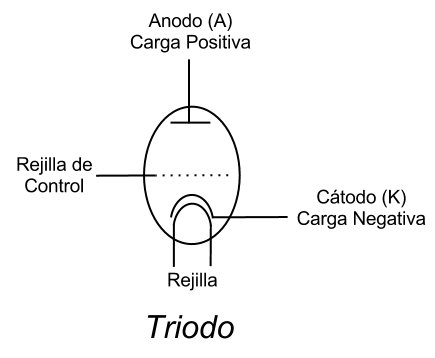
\includegraphics{images/triodo.png}
\caption{Triodo}
\end{figure}

La tensión aplicada a la rejilla hace que el flujo de electrones desde
el cátodo al ánodo sea mayor o menor. Esto es muy interesante pues
aplicando una señal de muy débil intensidad entre cátodo y rejilla
podemos conseguir que la variación del flujo de electrones entre éste y
el ánodo sea muy grande. Es decir, con una pequeña tensión controlamos
una gran corriente. A ese fenómeno se le llama amplificación. Por eso,
el triodo es un amplificador.

\subsection{Estructura básica.}\label{estructura-buxe1sica.}

El transistor consta de un sustrato (usualmente silicio) y tres partes
dopadas artificialmente (contaminadas con materiales específicos en
cantidades específicas) que forman dos uniones bipolares, el emisor que
emite portadores, el colector que los recibe o recolecta y la tercera,
que está intercalada entre las dos primeras, modula el paso de dichos
portadores (base).

\begin{figure}[htbp]
\centering
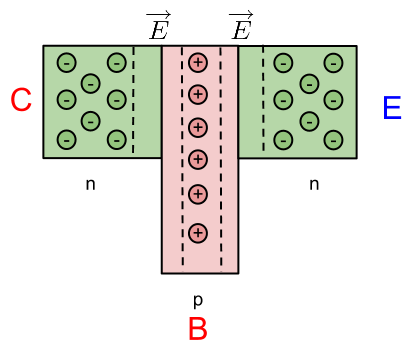
\includegraphics{images/bjt_base.png}
\caption{Estructura básica del BJT}
\end{figure}

A diferencia de las válvulas, el transistor es un dispositivo controlado
por corriente y del que se obtiene corriente amplificada. En el diseño
de circuitos a los transistores se les considera un elemento activo, a
diferencia de los resistores, condensadores e inductores que son
elementos pasivos. `'Su funcionamiento sólo puede explicarse mediante
mecánica cuántica.'`De manera simplificada, la corriente que circula por
el colector es función amplificada de la que se inyecta en el emisor,
pero el transistor sólo gradúa la corriente que circula a través de sí
mismo, si desde una fuente de corriente continua se alimenta la base
para que circule la carga por el colector, según el tipo de circuito que
se utilice. El factor de amplificación o ganancia logrado entre
corriente de colector y corriente de base, se denomina'`Beta del
transistor''.

\begin{equation}\label{eq:b}
\beta = \frac{i_{c}}{i_{b}}
\end{equation}

Otros parámetros a tener en cuenta y que son particulares de cada tipo
de transistor son:

\begin{itemize}
\itemsep1pt\parskip0pt\parsep0pt
\item
  Tensiones de ruptura de Colector Emisor.
\item
  Tensiones de ruptura de Base Emisor.
\item
  Tensiones de ruptura de Colector Base.
\item
  Potencia Máxima, disipación de calor.
\item
  Frecuencia de trabajo.
\end{itemize}

Además, de varias tablas donde se grafican los distintos parámetros
tales como corriente de base, tensión Colector Emisor, tensión Base
Emisor, corriente de Emisor, etc. Los tres tipos de
esquemas(configuraciones) básicos para utilización analógica de los
transistores son:

\begin{itemize}
\itemsep1pt\parskip0pt\parsep0pt
\item
  Emisor común.
\item
  Colector común.
\item
  Base común.
\end{itemize}

\subsection{Funcionamiento}\label{funcionamiento}

En una configuración normal, la unión emisor-base se polariza en directa
y la unión base-colector en inversa. Debido a la agitación térmica los
portadores de carga del emisor pueden atravesar la barrera de potencial
emisor-base y llegar a la base. A su vez, prácticamente todos los
portadores que llegaron son impulsados por el campo eléctrico que existe
entre la base y el colector.

Un transistor NPN puede ser considerado como dos diodos con la región
del ánodo compartida.

En una operación típica, la unión base-emisor está polarizada en directa
y la unión base-colector está polarizada en inversa. En un transistor
NPN, por ejemplo, cuando una tensión positiva es aplicada en la unión
base-emisor, el equilibrio entre los portadores generados térmicamente y
el campo eléctrico repelente de la región agotada se desbalancea,
permitiendo a los electrones excitados térmicamente inyectarse en la
región de la base. Estos electrones ``vagan'' a través de la base, desde
la región de alta concentración cercana al emisor hasta la región de
baja concentración cercana al colector. Estos electrones en la base son
llamados portadores minoritarios debido a que la base está dopada con
material P, los cuales generan ``huecos'' como portadores mayoritarios
en la base.

Utilizando la ley de Kirchhoff se tiene que;

\begin{equation}\label{eq:ie}
i_{e}=i_{c}+i_{b},
\end{equation}

sustituyendo \eqref{eq:b} en \eqref{eq:ie} se tiene que

\begin{equation}
i_{b}= \frac{i_{e}}{\beta +1}
\end{equation}

y

\begin{equation}
i_{c}= i_{e}\frac{\beta}{\beta +1}
\end{equation}

La región de la base en un transistor debe ser constructivamente
delgada, para que los portadores puedan difundirse a través de esta en
mucho menos tiempo que la vida útil del portador minoritario del
semiconductor, para minimizar el porcentaje de portadores que se
recombinan antes de alcanzar la unión base-colector. El espesor de la
base debe ser menor al ancho de difusión de los electrones.

    \subsection{Curvas Caracteristicas}\label{curvas-caracteristicas}

    \section{Circuito con un Transitor
BJT}\label{circuito-con-un-transitor-bjt}

\begin{center}\rule{3in}{0.4pt}\end{center}

Este es un circuito básico dentro del estudio de amplificadores con un
transistor con la teoria de amplificadores de baja potencia y baja
frecuencia.

Una de sus principales caracteristicas es la que se conoce como
\textbf{Insensibilidad a variaciones de la $\beta$}, la cual permite que
el comportamiento del circuito no varie significativamente ante pequeñas
variaciones de la $\beta$. Sin embargo, para lograr esto se requiere
cumplir ciertas condiciones que dificultan el diseño del circuito.

El esquema del circuito se muestra en la siguiente figura

De forma genera se puede considerar que el valor de los capacitores de
acoplo es muy grande (idelamente $X_{c}\rightarrow\infty$) de forma tal
que la impedancia del capacitor $X_{c}$ es:

\begin{equation}\label{eq:xc}
X_{c}= \begin{cases}
\infty    & w=0 \\\
0 &  w \neq 0
\end{cases}
\end{equation}

De la expresión \eqref{eq:xc}, entonces podemos concluir que la energía
proporcionada por la fuente de DC se encuentra contenido únicamente en
la parte del circuito relacionado con el transistor. Por lo tanto es
posible analizar el circuito considerando primero la fuente de DC y
luego agregar los efectos de la fuente de AC de forma similar al teorema
de superposición de fuentes, con la diferencia que al analizar el efecto
de la fuente de AC se considera que el transistor mantiene el efecto de
la fuente de DC llamado punto de operación $Q$.

    \subsection{Analisis de DC}\label{analisis-de-dc}

\begin{center}\rule{3in}{0.4pt}\end{center}

El circuito más simple con un transitor es el que se muestra en la
siguiente figura

Al analizar el circuito anterior por medio del analisís de mayas, se
tiene que:

de este circuito se obtienen para la maya $\color{blue}{1}$ la expresión
\eqref{eq:cir1may1}:

\begin{equation}\label{eq:cir1may1}
\color{blue}{V_{cc}=V_{R_{c}}+V_{ce}}
\end{equation}

del maya $\color{red}{2}$ se obtiene la expresión \eqref{eq:cir1may2}

\begin{equation}\label{eq:cir1may2}
\color{red}{V_{cc}=V_{R_{b}}+V_{be}}
\end{equation}

Si suponemos que el transistor se encuentra en la region lineal entonces
se tiene que:

\[
\begin{align}
\label{eq:ic} i_{c} &= \beta i_{b}  \\
\label{eq:Ie} i_{e} & = i_{c} + i_{b} \\
\label{eq:icIe} i_{e} & = \alpha i_{c}   \\ 
\label{eq:alhpa} \alpha & = \frac{\beta}{\beta+1} 
\end{align}
\]

Considerando la \textbf{ley de Ohm} en la expresión \eqref{eq:cir1may1}
se tiene que:

\begin{equation}\label{eq:cir1may1b}
\color{blue}{V_{cc}=i_{R_{c}}R_{c}+V_{ce}}
\end{equation}

dado que la resistencia $R_{c}$ esta en serie con el transitor, entonces
se puede considerar que $\color{green}{i_{c}=i_{R_{c}}}$, por lo que la
expresión \eqref{eq:cir1may1b} se puede reescribir como:

\begin{equation}\label{eq:cir1may1c}
\color{blue}{V_{cc}=i_{c}R_{c}+V_{ce}}
\end{equation}

En la expresión \eqref{eq:cir1may1c} se tiene que $i_{c}$ y $V_{ce}$ son
parámetros del transistor y por lo tanto se consideran incognitas, lo
cual lleva a que no se pude encontrar una solución única. Utilizando un
analisís similar en la expresión \eqref{eq:cir1may2} se tiene que:

\begin{equation}\label{eq:cir1may2a}
\color{red}{V_{cc}=i_{b}R_{b}+V_{be}}
\end{equation}

En la expresión \eqref{eq:cir1may2a} se tiene que idelamente en un
transistor de silicio $V_{be}=0.7$, por lo que se tiene que:

\begin{equation}\label{eq:cir1may2b}
\color{red}{i_{b}=\frac{V_{cc}+V_{be}}{R_{b}}}
\end{equation}

De la expreesión \eqref{eq:cir1may2b} se observa que el valor de la
corriente $i_{b}$ es determinado por elementos externos al transistor
($V_{cc}$ y $R_{b}$). Además, si se considera la expresión \eqref{eq:ic}
en \eqref{eq:cir1may1c} entonces se tiene que el valor de $i_{c}$ y de
$V_{ce}$ se determinán por los elementos externos al tranistor.

Si los elemento externos determinan los posibles valores de los
parámetros del transistor ($i_{b}$,$i_{c}$ y $V_{ce}$) entonces, sin
importar el valor de $\beta$ se puede representar graficamente cualquier
posible valor de $i_{c}$ y $V_{ce}$ utilizando la expresión
\eqref{eq:cir1may1c}, se tiene que el máximo valor de $i_{c}$ se obtiene
cuando $V_{cc}=0$ y su expresión es:

\begin{equation}\label{eq:cir1icmax}
\color{blue}{i_{c}=\frac{V_{cc}}{R_{c}}}
\end{equation}

el valor máximo de $V_{ce}$ se obitene cuando $i_{c}=0$ y su expresión
es:

\begin{equation}\label{eq:cir1vccmax}
\color{blue}{V_{ce}=V_{cc}}
\end{equation}

De las expresiones \eqref{eq:cir1may1c},\eqref{eq:cir1icmax} y
\eqref{eq:cir1vccmax} se puede concluir que un incremento en $i_{c}$ o
$V_{ce}$ involucra un decremento en $V_{ce}$ o $i_{c}$ respectivemente.
Dado que el transitor trabaja en el primer cuadrante de la grafica IV,
entonces todo posible valor de $i_{c}$ y $V_{ce}$ se puede representar a
través de la siguiente gráfica

La recta en la figura anterior es conocida como \textbf{Recta de Carga},
la cual se puede definir como: \textbf{La representación gráfica de
todos los posibles valores de $i_{c}$ y $V_{ce}$}. La Recta de carga,
junto con las curvas caracteristicas del transistor nos permiten
determinar el comportamiento del circuito, al poder determinar si en que
región de funcionamiento se encuentra el transistor, es importante
recordar una de las hipotesis en el analisís es considerar que el
transistor se encuentra en la región lineal.

Aunque la Recta de Carga representa todos los posibles valores de
$i_{c}$ y $V_{ce}$, en la práctica se tiene que $i_{c}$ y $V_{ce}$
tienen un valor único, debido a que todos los elementos en el cicruito
se considera que tienen un valor constante, a ese valor especifico de
$i_{c}$ y $V_{ce}$ debido a los valores del circuito se le llama
\textbf{Punto de Operación}.

Dadas las expresiones \eqref{eq:ic} y \eqref{eq:cir1may1c} se puede
considerar que $V_{ce}$ es una señal de AC con un componente de DC (una
señal de AC con un offset) considerar que $i_{c}$ y $V_{ce}$. El punto
de operación cuando la señal de AC es nula corresponde al compente de
DC, y se llama \textbf{punto de reposo} es denota con la letra $Q$. En
la siguiente figura se presenta un bosquejo de la evolución en tiempo de
$V_{ce}$.

La amplitud de la señal $V_{ce}$ está limitado por la expresión
\eqref{eq:cir1vccmax} y la naturaleza del transitor que requiere que
$V_{ce}\geq0$ por lo que se tiene que:

\begin{equation}\label{eq:vceac}
0\leq V_{ce}(AC) \leq V_{cc}
\end{equation}

Dado que el comportamiento de $V_{ce}$ esta relacionado con $i_{c}$ por
la expresión eqref\{eq:cir1may1c\}, entoces se concluye que $i_{c}$
presente un comporamiento similar a $V_{ce}$ pero de forma inversa,
cuando $V_{ce}$ aumenta $i_{c}$ disminuye. Si consideramos el
comportamiento de AC sobre la recta de carga, se tendra que el punto de
reposo es el origen del sistema de AC. Además que los limites del
comportamiento de AC por la expresión \eqref{eq:vceac} y de forma
similar $i_{c}$ por:

\begin{equation}\label{eq:icac}
0\leq i_{c}(AC) \leq \frac{V_{cc}}{R_{c}}
\end{equation}

graficamente se representa en la siguiente figura

    \[\color{blue}{
\begin{eqnarray}
V_{TH} &= & V_{R_{i}}+V_{BE}+V_{R_{E}} \\\
V_{CC} &= & V_{R_{C}}+V_{CE}+V_{R_{E}} 
\end{eqnarray}}\]


    % Add a bibliography block to the postdoc
    
    
    
    \end{document}
